\documentclass[12pt]{article}
 
\usepackage[margin=1in]{geometry} 
\usepackage{amsmath,amsthm,amssymb}
\usepackage{float}
\usepackage{tikz}
\usetikzlibrary{arrows,shapes,trees} % loads some tikz extensions
 
\begin{document}
 
\title{Homework 3}
\author{Josh Klontz
CSE 802}
 
\maketitle

\begin{enumerate}
\item \textbf{Solve the following problems from Chapter 3 of the textbook: 1, 10, 17, 19}
\subitem \textbf{1. Let $x$ have an exponential density}
  \begin{equation}
    p(x|\theta) = \left\{\begin{array}{ll}\theta e^{-\theta x}&x\geq 0\\0&otherwise\end{array}\right.
  \end{equation}
  \begin{enumerate}
  \item \textbf{Plot $p(x|\theta)$ versus $x$ for $\theta = 1$. Plot $p(x|\theta)$ versus $\theta$, $(0 \leq \theta \leq 5)$, for $x=2$.}
    \begin{equation}
      p(x|1) = \left\{\begin{array}{ll} e^{-x}&x\geq 0\\0&otherwise\end{array}\right.
    \end{equation}
    \begin{figure}[H]
      \centering
      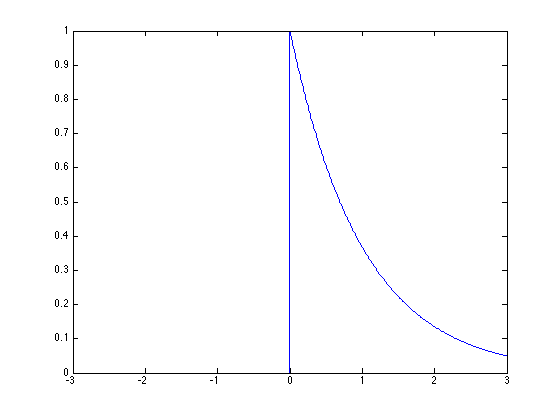
\includegraphics[width=4in]{1a1}
      \caption{$p(x|\theta)$ versus $x$ for $\theta = 1$.}
    \end{figure}
  \begin{equation}
    p(2|\theta) = \theta e^{-2\theta}
  \end{equation}
  \begin{figure}[H]
      \centering
      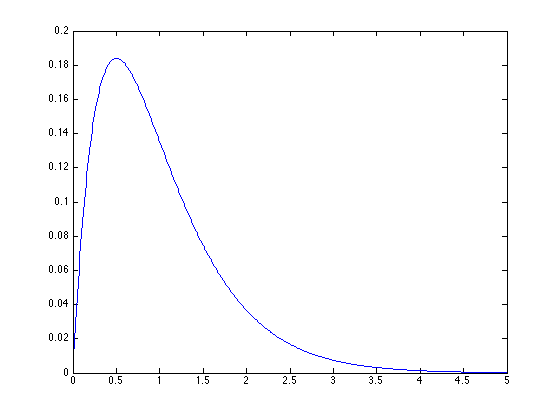
\includegraphics[width=4in]{1a2}
      \caption{$p(x|\theta)$ versus $\theta$, $(0 \leq \theta \leq 5)$, for $x=2$.}
    \end{figure}
  \item \textbf{Suppose that $n$ samples $x_1,...,x_n$ are drawn independently according to $p(x|\theta)$. Show that the maximum likelihood estimate for $\theta$ is given by}
    \begin{equation}
      \hat{\theta} = \frac{1}{\frac{1}{n}\sum_{k=1}^nx_k}
    \end{equation}
    \begin{equation}
    \begin{split}
      p(D|\theta)& = \prod_{k=1}^n p(x_k|\theta) \\
      & = \prod_{k=1}^n \left\{\begin{array}{ll}\theta e^{-\theta x_k}&x_k\geq 0\\0&otherwise\end{array}\right. \\
      & = \prod_{k=1}^n \theta e^{-\theta x_k} \\
      & = \theta^n \prod_{k=1}^n e^{-\theta x_k} \\
      & = \theta^n e^{-\theta \sum_{k=1}^n x_k} \\
      0& = ln(p(D|\theta))^\prime \\
      & = ln(\theta^n e^{-\theta \sum_{k=1}^n x_k})^\prime \\
      & = ln(\theta^n)^\prime - (\theta \sum_{k=1}^n x_k)^\prime \\
      & = \frac{n}{\theta} - \sum_{k=1}^n x_k \\
      \hat{\theta}& = \frac{n}{\sum_{k=1}^nx_k} \\
      & = \frac{1}{\frac{1}{n}\sum_{k=1}^nx_k} \\
      & \qed
    \end{split}
    \end{equation}
  \item \textbf{On your graph generated with $\theta = 1$ in part (a), mark the maximum likelihood estimate $\hat{\theta}$ for large $n$.}
    \begin{equation}
    \begin{split}
      \hat{\theta}& = \frac{1}{\frac{1}{n}\sum_{k=1}^nx_k} \\
      & \approx \frac{1}{\bar{x}} \\
      & = \frac{1}{\int_0^\infty e^{-x} dx} \\
      & = \frac{1}{-e^{-x}|_0^\infty} \\
      & = \frac{1}{-e^{-\infty} - -e^{-0}} \\
      & = \frac{1}{0 + 1} \\
      & = 1 \\
    \end{split}
    \end{equation}
    \begin{figure}[H]
      \centering
      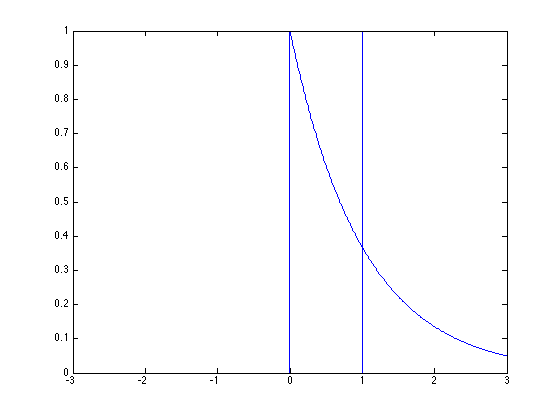
\includegraphics[width=4in]{1c}
      \caption{$p(x|\theta)$ versus $x$ for $\theta = 1$. $\hat{\theta} = 1$.}
    \end{figure}
  \end{enumerate}
  \subitem \textbf{10. Suppose we employ a novel method for estimating the mean of a data set $D = \{x_1,x_2,...,x_n\}$: We assign the mean to be the value of the first point in the set, that is, $x_1$.}
  \begin{enumerate}
  \item \textbf{Show that this method is unbiased.} \\
    The method is \emph{unbiased} if the expected value over all data sets of size $n$ is equal to the true mean.
    \begin{equation}
    \begin{split}
      D& = \{x_1,x_2,...,x_n\} \\
      \theta(D)& = x_1 \\
      E(\theta(D))& = \frac{\sum_{k=0}^{n!} \theta(permutation_k(D))}{n!} \\
      & = \frac{\sum_{i=0}^{n} x_i \cdot (n-1)!}{n \cdot (n-1)!} \\
      & = \frac{1}{n}\sum_{i=0}^{n} x_i \\
      & \qed
    \end{split}
    \end{equation}
  \item \textbf{State why this method is nevertheless highly undesirable.} \\
  This method is highly undesirable because the error of the method is equal to the variance of the data. A much more stable estimate of the mean can be computed by actually taking the average of all the data points.
  \end{enumerate}
\end{enumerate}

\end{document}
